\chapter{中微子探测器的模拟框架}
\label{chap:simulation_framework}

对高能中微子的反应以及其探测过程的模拟是极其复杂的,因为其中包含多种不同能量尺度的物理过程::初始中微子和DIS顶点产生的主要次级粒子在在$\mathrm{TeV} - \mathrm{PeV}$量级,簇射演化时发生的级联过程会产生大量的$\mathrm{MeV} - \mathrm{GeV}$能级的次级粒子,而这些带电粒子产生的切伦科夫光子在$\mathrm{eV}$量级。
高能中微子反应与其探测过程中的各个粒子的自由程也各不相同:初始中微子可以穿透整个地球,而其DIS反应引发的粒子簇射中的粒子在海水中的自由程大约为$1\,\mathrm{cm}$(低能电子)$-100\,\mathrm{cm}$(高能光子),形成的整个粒子簇射的大小大长约$10\,\mathrm{m}$,半径约$0.1\,\mathrm{cm}$(电磁簇射)$-10\,\mathrm{cm}$(强子簇射),缪子在海水中的传播可以延伸至约$1\,\mathrm{km} - 10\,\mathrm{km}$,切伦科夫光子的传播由光的吸收长度所限制,大约局域在$\lesssim 100\, \mathrm{m}$的范围内。
因此,我们将中微子事件和探测器响应的模拟过程分为多个不同的模块,每个模块负责处理一部分的物理过程。在下面的章节中,我们对各个模拟模块进行介绍。

\section{中微子事件产生器}
\label{sec:event_generator}

中微子事件产生器(event generator)为后续的探测器模拟注入初始粒子,它主要进行以下任务:
\begin{enumerate}
    \item 模拟中微子与原子核的DIS作用
    \item 模拟陶中微子的衰变过程
    \item 模拟粒子从望远镜阵列外传播到阵列的过程
    \item 进行带权重的重要性采样
\end{enumerate}

由于中微子事件产生器要处理的任务复杂,各个中微子望远镜的合作组都为自己的实验设计了一套对应的模拟程序,例如\textsf{ANIS}\cite{ANIS:2004},\textsf{gSeaGen}\cite{gSeaGen:2020},\textsf{LeptonInjector-LeptonWeighter}\cite{LeptonInjector:2020}等。
海铃合作组也同样设计了一套中微子事件产生器\footnote{\url{https://gitlab.com/hailing/event-generator}},它是基于\textsf{CORSIKA8}模拟框架\cite{CORSIKA8:2018, CORSIKA8:2022}实现的。
\textsf{CORSIKA8}是著名宇宙线级联过程模拟软件\textsf{CORSIKA7}\cite{CORSIKA7:1998}的C++重构版本,它具有更好的可拓展性,用户可以更为轻易地通过C++接口添加感兴趣的物理过程并添加形状更复杂的探测器。
借助于\textsf{CORSIKA8}模拟框架,我们得以实现了中微子事件产生器所要求的各项功能,并且在该模拟框架下制作的程序具有更好的模块化特点,便于后期的更新和维护。

事件产生器的输入为我们要采样的初始中微子的动力学范围,例如中微子的能谱和方向,以及感兴趣的探测器范围等。程序的输入配置以\textsf{json}的格式进行保存,方便用户查看和修改。
事件产生器最终的输出结果为一系列的\textsf{McEvent}类的对象,它类似于粒子物理中常用的\textsf{HepMC3}蒙特卡洛输出结果\cite{HepMC3:2019},包含粒子物理事件的顶点和产物的动力学信息。具体的来说,每一个事件中都包含初始中微子的信息,DIS反应得到的初始粒子的信息,把这里粒子传播到达探测器表面后得到的新粒子信息,以及该事件的权重。
输出结果目前是以\textsf{json}的格式保存,这样可以方便人类用户直接查看事件中的数据,并且具有很好的可拓展性,但缺点是空间和时间上的效率相比于二进制文件来说低很多。

\subsection{几何设置}

\textsf{CORSIKA8}模拟框架中支持几种基本几何体,如球形,长方体,圆柱体等。在设置了几何体的形状后,还可以为其设置原子组分,介质密度,电离能损等信息,用于支持后续的物理过程模拟。
我们在\textsf{CORSIKA8}中构建了一个地球的密度模型,并且在其中放置了一个圆柱形粒子探测区域,用于表示海铃中微子探测器,如图\ref{fig:corsika_geometry}中所示。
我们采用了PREM(preliminary reference Earth model)\cite{PREM:1981}来对地球的密度分布进行建模,其密度模型如图\ref{fig:prem}所示。
在此基础上,我们添加了一层$3.4\,\mathrm{km}$厚的海水包裹在地壳外围,用于表示海铃所在位置的海水深度。
海铃中微子探测器的粒子检测范围为一个半径$2500\,\mathrm{m}$,高度$1000\,\mathrm{m}$的圆柱体。当粒子进入该圆柱体之后,\textsf{CORSIKA8}将不再继续进行粒子传播模拟,而是将粒子保存下来,作为后续更为精细的探测器模拟的输入。

\begin{figure}[htb]
\centering
    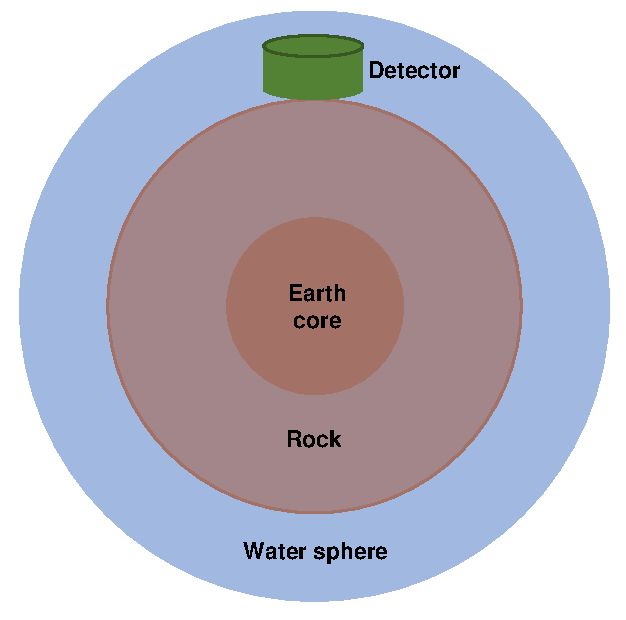
\includegraphics[width=0.70\textwidth]{img/corsika_geometry.pdf}
    \caption{模拟中的几何示意图。}
    \label{fig:corsika_geometry}
\end{figure}

\begin{figure}[htb]
\centering
    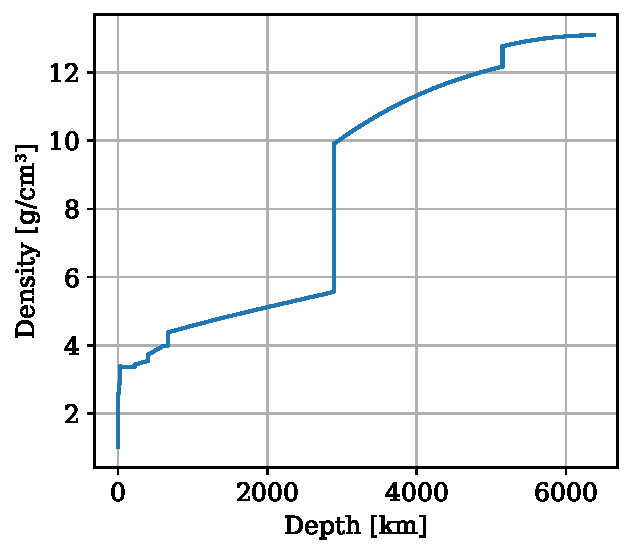
\includegraphics[width=0.60\textwidth]{img/prem.pdf}
    \caption{地球的密度模型。}
    \label{fig:prem}
\end{figure}

\subsection{DIS反应顶点的模拟}

在我们的模拟框架中,DIS和陶中微子的衰变过程都是通过\textsf{PYTHIA-8.3}程序\cite{Pythia8.2:2014, Pythia8.3:2022}实现的。
\textsf{PYTHIA}主要应用在大型强子对撞机(large hadron collider, LHC)中来模拟质子-质子碰撞后产生的结果,如图\ref{fig:event_generator_schem}所示。
除了强子-强子对撞模拟外,\textsf{PYTHIA}还可以处理轻子-轻子和轻子-强子对撞,以及粒子衰变的模拟。

\begin{figure}[htb]
\centering
    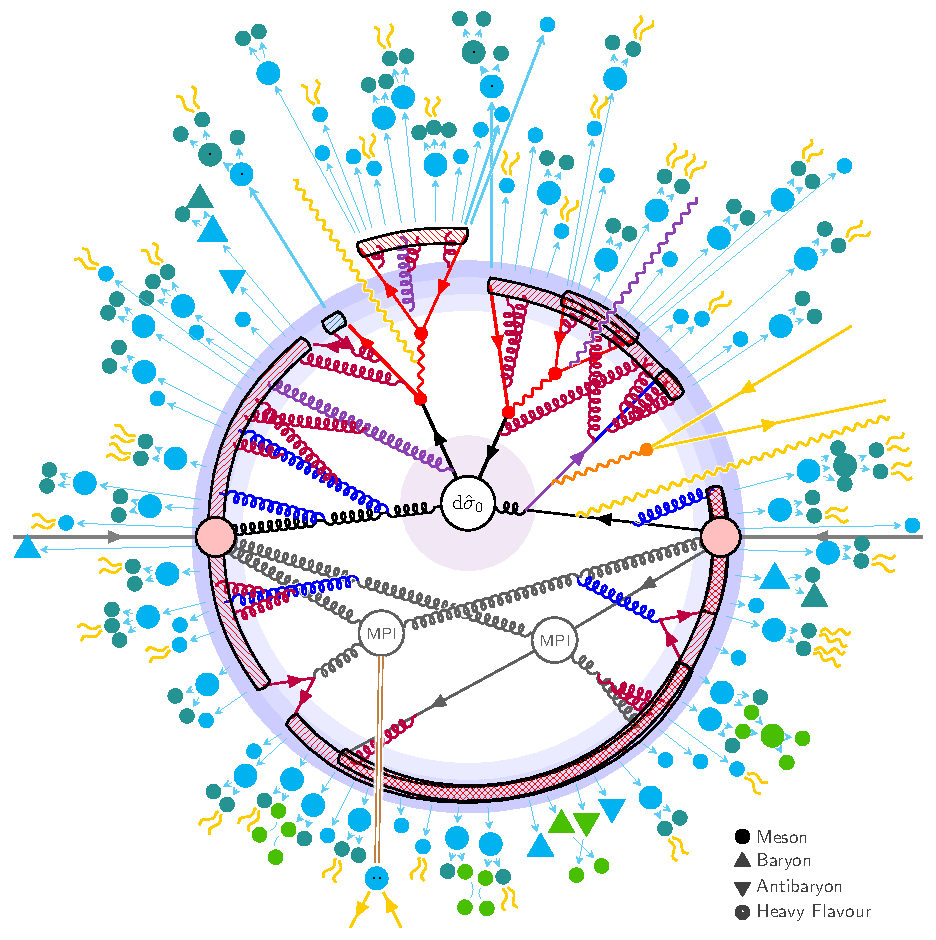
\includegraphics[width=0.73\textwidth]{img/event_generator_schem_fig.pdf}
    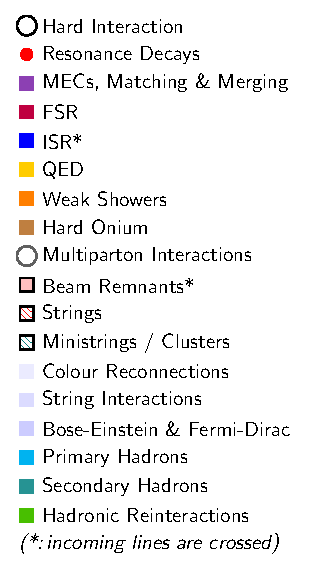
\includegraphics[width=0.25\textwidth]{img/event_generator_schem_legend.pdf}
    \caption{\textsf{PYTHIA}所处理的$pp\to t\bar{t}$事件的示意图。}
    \label{fig:event_generator_schem}
\end{figure}

用Pythia模拟中微子与原子核的DIS过程在Pythia程序内的反应分类中属于轻子-强子反应这一类别。在应用时,我们只需要打开Pythia程序中有关带电流相互作用的设置,再输入中微子的能动量信息以及靶粒子的信息,即可让Pythia进行DIS过程的模拟。
在我们的模拟框架中,我们在\textsf{CORSIKA8}中接入\textsf{PYTHIA}物理反应模块,将中微子传递到\textsf{PYTHIA}来进行DIS反应后,再将反应得到的粒子产物传回\textsf{CORSIKA8}中的栈堆,然后再进行后续的模拟。
通过Pythia模拟得到的$1\,\mathrm{PeV}$的电子中微子与质子发生DIS作用后得到的产物能量分布如图\ref{fig:DIS_product_energy_dist_primary}和\ref{fig:DIS_product_energy_dist_secondary}中所示。

\begin{figure}[!ht]
\centering
    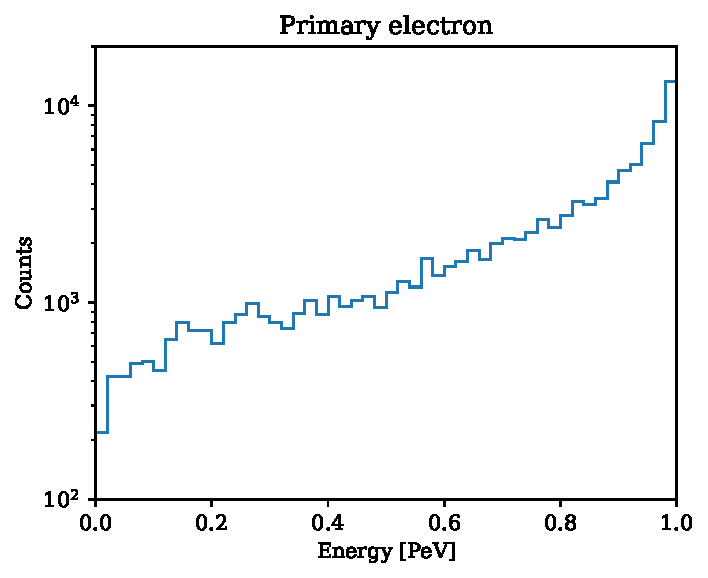
\includegraphics[width=0.60\textwidth]{img/DIS_primary_electron.pdf}
    \caption{在\textsf{Pythia}程序中模拟100k次$1\,\mathrm{PeV}$的电子中微子与质子发生带电流的DIS过程后,带电流作用中产生的主电子的能量分布图。}
    \label{fig:DIS_product_energy_dist_primary}
\end{figure}

\begin{figure}[!ht]
\centering
    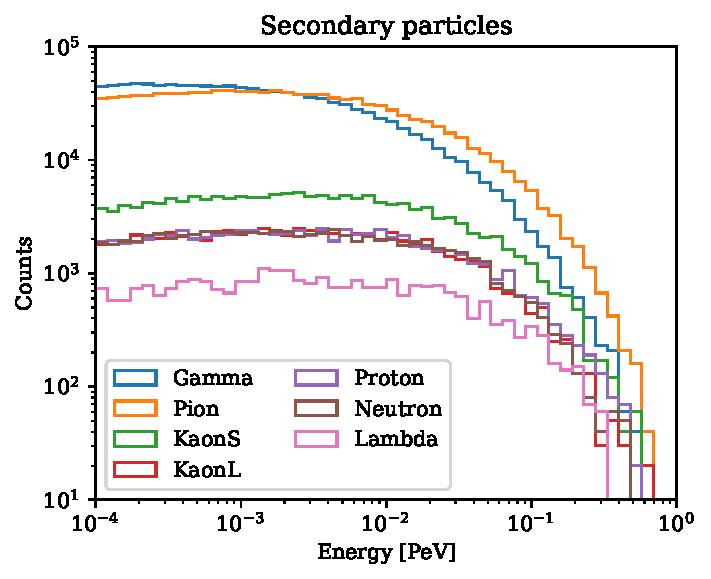
\includegraphics[width=0.60\textwidth]{img/DIS_secondary_particles.pdf}
    \caption{在\textsf{Pythia}程序中模拟100k次$1\,\mathrm{PeV}$的电子中微子与质子发生带电流的DIS过程后,原子核碎裂产生的主要成分的分布。}
    \label{fig:DIS_product_energy_dist_secondary}
\end{figure}


\subsection{缪子中微子径迹型事件采样}
\label{subsec:muon_sampling}

缪子可以在海水中传播$\mathcal{O}(10\,\mathrm{km})$,因此在距离探测器较远处的位置发生的DIS产生的缪子同样有可能传播到探测器,形成径迹型事件。
此类事件的反应顶点位置和方向的采样比较复杂,我们采用类似IceCube中的模拟程序\textsf{LeptonInjector-LeptonWeighter}\cite{LeptonInjector:2020}的采样模式。

该采样模式大致分为以下几步:
\begin{enumerate}
    \item 根据一个感兴趣的中微子能谱$F_\mathrm{mc}(E_\nu)$来对中微子的能量进行采样,得到中微子能量$E_\nu$。
    \item 在$4\pi$的立体角中随机选取一个方向$\vec{n}_\nu$,该方向将作为中微子的方向。
    \item 以探测器的中心为圆心,$R_0=2500\,\mathrm{m}$为半径(半径等同于探测器的大小),$\vec{n}_\nu$为法线方向,构成的圆盘中,均匀地抽取出一个点$\vec{x}_{i}$来作为中微子的初始位置。
    \item 调用\textsf{Pythia-8.3}物理模块来模拟该中微子与原子核的带电流的DIS反应过程,得到反应的产物,其中将会包含一个高能缪子。
    \item 通过缪子能损公式,来估计缪子能量$E_\mu$所对应能传播的柱密度范围$X_\mu$。
    \item 朝着中微子方向的反方向$-\vec{n}_\nu$,发射一条射线,计算该射线上柱密度达到$X_\mu$的地方到射线原点的距离,记为$D_\mu$。该过程中将会涉及到地球的密度模型,如果当射线超出地球范围时柱密度已然没有达到$X_\mu$,则进行截断。
    \item 在以$\vec{x}_\mathrm{i}$为原点,$\vec{n}_\nu$为方向,长度范围为$(-D_\mu-D_0, D_0)$的线段上均匀抽样出一个点$\vec{x}_\mathrm{f}$,这个点将会被作为真实反应发生的点,中微子和此前DIS产生的粒子的位置都将被设置在该点处。其中$D_0 = 2500\,\mathrm{m}$是一个与探测器大小接近的量,这里我们要求上述构造的长度范围为$(-D_\mu-D_0, D_0)$的线段足以包含以$\vec{x}_\mathrm{i}$为原点,$\vec{n}_\nu$为方向所构造的直线与探测器的相交线段。同样的,此时如果有线段超出地球的范围,就会进行响应的截断。
\end{enumerate}

通过以上的采样过程,我们的采样范围足以覆盖所有能够被探测器探测到的径迹型事件的反应顶点和方向,而与此同时,我们也并没有浪费计算资源模拟过多的无法被探测器检测到的信号,这样的蒙特卡洛采样在计算性能上是相当优秀的。

该采样过程对初始中微子的能量$E_\nu$,方向$\hat{n}_\nu$,和反应的顶点位置$x_\mathrm{f}$这三个维度进行了采样,而且其中很多过程都是均匀采样的。
然而真实的物理过程在该三个维度上的分布并非如此,例如中微子在探测器附近的流量大小与其真实流量以及穿过地球的概率有关,中微子的反应位置分布与探测器附近的密度分布有关,等等。
为了将我们采样的结果与这些物理过程联系起来,我们需要引入采样权重的概念,这种带权重的采样过程称为重要性采样。有关权重的内容,我们将会在\ref{subsec:weightings}中详细讨论。

如上所述,我们的事件产生器模拟的结果便是一系列的中微子DIS事件在探测器上的结果,以及对应的权重项。

\subsection{缪子传播模拟}

在此前的几节内容中,我们介绍了如何通过\textsf{Pythia8}来模拟缪子中微子与原子核的DIS过程,并且还介绍了如何采样这些DIS事件在中微子能量,方向和顶点位置这些相空间上的分布。对于缪子中微子通过带电流的形式发生的DIS作用而言,其产生的缪子可以传播公里到数十公里的量级。此时如果DIS顶点发生在探测器外,则需要将产生的缪子传播到探测器,即进行缪子传播过程的模拟。

在我们的模拟框架中,我们采用\textsf{PROPOSAL}程序来模拟缪子和其他轻子的传播过程\cite{PROPOSAL:2013, PROPOSAL:2019}。
在传播经过$100\,\mathrm{m}$的海水时,不同能量的缪子损失的平均能量如图\ref{fig:muon_energy_loss}中所示,可以看到在$1\,\mathrm{TeV}$的能量以上时,缪子的能损是辐射形式主导的,即能损效率正比于自身的能量,其对应的物理过程主要包括韧致辐射,正负电子对产生和光核反应。
这种辐射形式的能损过程具有散射截面小,沉积能量的范围波动大的特点,其能损过程可以引发伴随的电磁簇射或者强子簇射,因此具有具有很强的不确定性。
图\ref{fig:muon_energy_loss_hist}展示了各个能量下缪子穿行$100\,\mathrm{m}$的海水时损失能量的分布,可以看到在极端的情况下,缪子可以将自身几乎全部的能量都沉积其中。

\begin{figure}[!ht]
\centering
    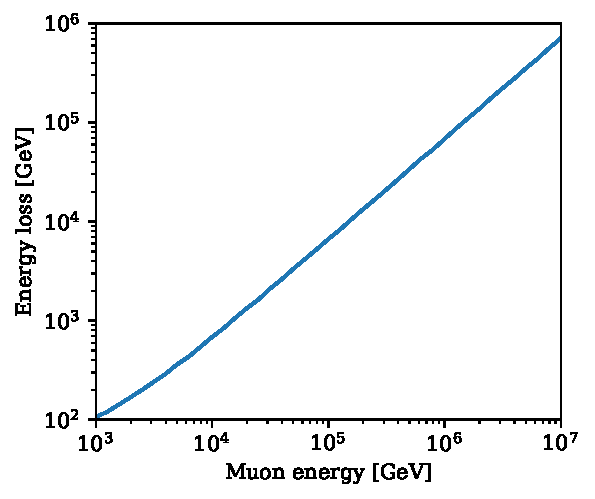
\includegraphics[width=0.55\textwidth]{img/muon_energy_loss.pdf}
    \caption{不同能量下,缪子穿行$100\,\mathrm{m}$的海水时的平均能损。}
    \label{fig:muon_energy_loss}
\end{figure}

\begin{figure}[!ht]
\centering
    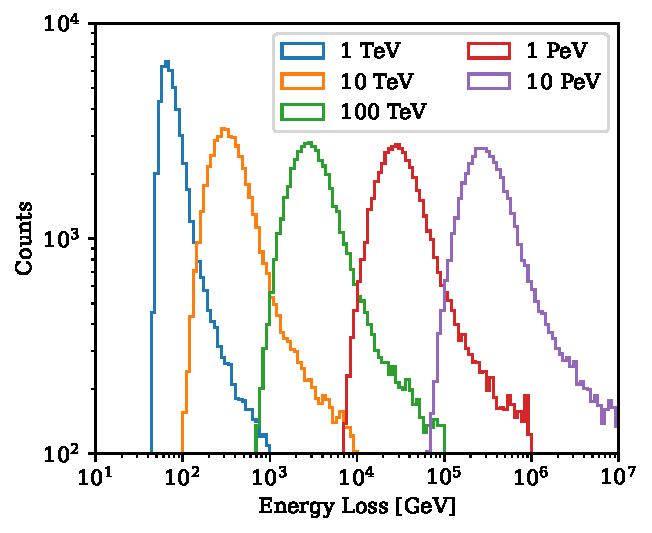
\includegraphics[width=0.60\textwidth]{img/muon_energy_loss_hist.pdf}
    \caption{不同能量下,缪子穿行$100\,\mathrm{m}$的海水时的能损分布。}
    \label{fig:muon_energy_loss_hist}
\end{figure}




\section{望远镜阵列内的粒子簇射模拟}
\label{sec:shower_simulation}

在使用中微子事件产生器生成探测器处能够接收到的粒子之后,我们将使用探测器模拟程序来继续模拟这些粒子的物理过程,进而得到真正对探测器而言能够探测到的物理信号,即光子在光敏元件上产生的光电子信号。

\subsection{高精度粒子物理过程模拟}

我们使用\textsf{Geant4}粒子模拟软件框架\cite{GEANT4:2003,GEANT4:2006}来对探测器内发生的粒子物理过程进行模拟。
\textsf{Geant4}中内置的物理库已经包含了从$\mathrm{eV}$到$100\,\mathrm{TeV}$能量范围内的绝大多数的粒子物理过程。
相比于\textsf{CORSIKA8},\textsf{Geant4}在低能范围内的物理准确性和计算效率都更为高效,而且其用户接口也更加丰富,适合进行详细的探测器内部模拟。

在我们的模拟中,我们将电子在海水中的簇射演化过程的动能阈值设置为$E_\mathrm{cut} = 0.25\,\mathrm{MeV}$,约等于电子在水中的切伦科夫能量阈值。这是为了保证所有能够产生切伦科夫光的粒子都被我们进行了模拟,确保事件的光产额不会丢失。


\subsection{通过参数化的方式加速簇射模拟}

电子在海水中主要通过韧致辐射和电离两种方式损失能量。其中韧致辐射过程将会发射光子,光子将会继续以康普顿散射的形式将能量传递给新的电子,由此实现了电子数量的倍增,即引发级联簇射过程。而电离过程会导致电子能量以热能的形式沉积在海水中,并在电子能量比较低时占据主要能损的地位。

在海水中,韧致辐射能损和电离能损的效率相同时的电子能量被定义为电子在海水中的临界能量(critical energy)\cite{PROPOSAL:2013}$E_c^e \simeq 0.1 \,\mathrm{GeV}$。\CHECK{CHECK THIS IN PROPOSAL}当电子能量高于$E_c^e$时将会发生级联簇射过程,而低于$E_c$时则不大可能会继续产生新的高能电子。
通过简单的计算,我们可以知道电子在海水中的簇射演化过程大约能产生的次级粒子数量为:
\begin{equation}
    N(E_0) \simeq E_0 / E_c^e
    \label{eq:param_flow_chart}
\end{equation}
其中$E_0$表示初始电子的能量。根据上述式子我们可以得到,对于约$100\,\mathrm{GeV}$的初始电子而言,其产生的次级电子数量可以达到$\sim 1000$个。
并且这些次级电子可以通过电离作用产生更多的低能电子,通过Geant4模拟中,我们可以统计到$\sim 20'000$个能量高于切伦科夫阈值($0.25\,\mathrm{MeV}$)的电子通过电离过程产生。
所有这些高于切伦科夫能量阈值的电子都可以辐射切伦科夫光子。

通过逐个粒子地方式模拟如此簇射演化中产生的大量的次级粒子将消耗不少的计算资源。在中微子望远镜中,几乎所有的电子级联过程都发生在空旷的海水中,因此簇射演化的过程实际上是比较稳定的。
图\ref{fig:param_num_photon_vs_energy}展示了电磁簇射中产生的总切伦科夫光子数与入射的电子能量之间的关系,我们可以看到他们之间存在如公式\ref{eq:emission_efficiency}中所描述的线性关系。
图\ref{fig:param_X_distribution}展示了电磁簇射的纵向发展,即产生切伦科夫光子的位置分布。
更多有关电磁簇射中物理量的分布和其拟合结果将在附录\ref{appendix:shower_param}中展示。

\begin{figure}[!ht]
\centering
    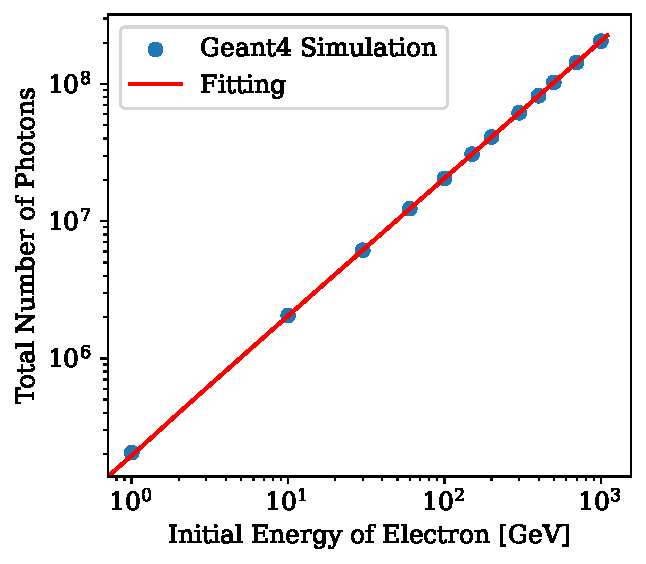
\includegraphics[width=0.65\textwidth]{img/param_num_photon_vs_energy.pdf}
    \caption{电磁簇射过程产生的总切伦科夫光子数与入射电子能量之间的关系图。}
    \label{fig:param_num_photon_vs_energy}
\end{figure}

\begin{figure}[!ht]
\centering
    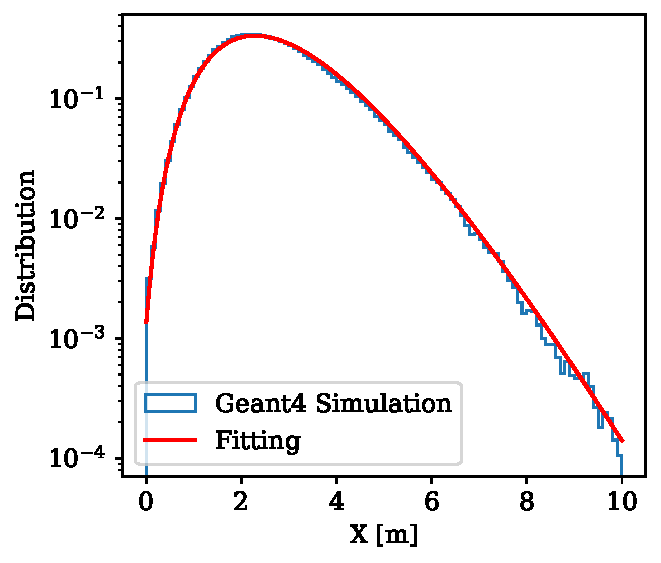
\includegraphics[width=0.65\textwidth]{img/param_X_distribution.pdf}
    \caption{电磁簇射过程中辐射切伦科夫光子的纵向分布。}
    \label{fig:param_X_distribution}
\end{figure}





通过对Geant4模拟实验的归纳总结,我们可以用参数化的方式来取代Geant4逐个粒子的模拟。
簇射过程参数化的程序结构示意图\ref{fig:param_flow_chart}所示。
考虑到中微子望远镜中实际的可观测量是切伦科夫光子,而切伦科夫光子是由带电粒子的轨迹所产生的,因此我们对电磁簇射演化过程进行参数化的目标便是快速得到一些能够产生切伦科夫光的轨迹,在我们的模拟中定义为\textsf{CherenkovStep},它包含带电粒子轨迹的运动信息(时间,位置,方向,速度)以及能够产生的切伦科夫光子的数量。
我们设计的级联过程参数化模块被嵌入到探测器模拟流程中,捕获能量在$1\,\mathrm{GeV}$到$100\,\mathrm{GeV}$能量范围内的电子,然后用参数化的方式将其快速转换为一系列的\textsf{CherenkovStep},从而取代标准的粒子物理模拟。

\begin{figure}[!ht]
\centering
    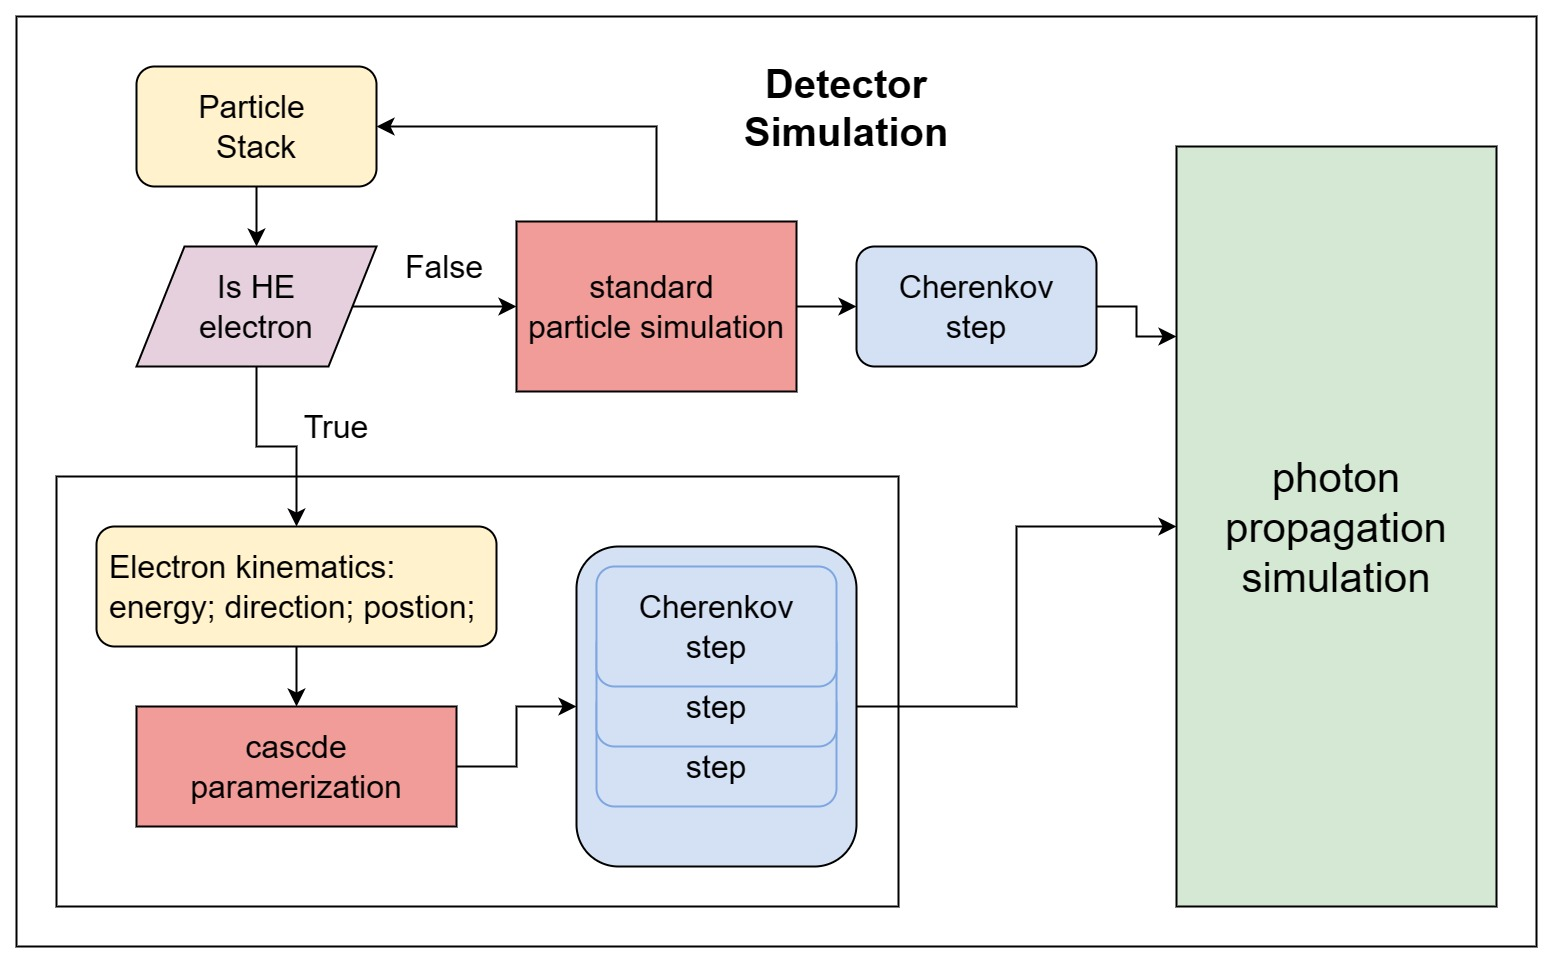
\includegraphics[width=0.95\textwidth]{img/param_flow_chart.jpg}
    \caption{簇射过程参数化的流程示意图。}
    \label{fig:param_flow_chart}
\end{figure}

\begin{figure}[!ht]
\centering
    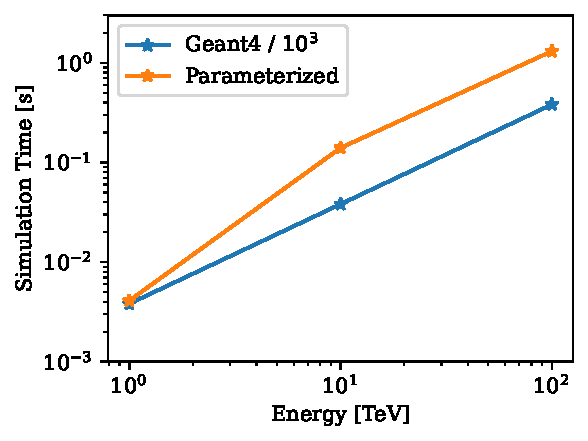
\includegraphics[width=0.65\textwidth]{img/performance_param.pdf}
    \caption{参数化的方式进行级联模拟与传统逐个粒子的模拟运行效率对比。}
    \label{fig:performance_param}
\end{figure}

通过参数化的方式进行级联模拟与传统逐个粒子的模拟运行效率对比如图\ref{fig:performance_param}所示。可以发现对于能量比较高的电子,以参数化的形式模拟之后,模拟速度有了$\mathcal{O}(1e^3)$倍的提升。

尽管簇射过程的参数化模拟无法做到和标准粒子物理流程得到的结果完全一致,我们的模拟研究表明,两者在光产额上的差距小于$1\%$,在DOM探测到的光子到达时间分布上差距小于$0.5\,\mathrm{ns}$。
这样的精度足以用于对中微子望远镜的性能研究,而参数化给模拟带来的性能提升是极其关键的,例如对于现代深度学习中的训练往往需要大量的模拟样本,只有使用参数化才有可能满足样本数量的需求。


\subsection{使用CORSIKA8来进行高能段的粒子过程模拟}

由于\textsf{Geant4}的强相互作用库只能进行实验室系下$100\,\mathrm{TeV}$能量的强子过程的模拟,不足以覆盖中微子望远镜中极高能部分的物理情形。
因此在将来的模拟框架中,我们将会使用\textsf{CORSIKA8}来代替\textsf{Geant4}来进行探测器内部的粒子物理过程模拟。
下面我们展示利用\textsf{CORSIKA8}来进行海水中的粒子级联过程的模拟结果


\section{切伦科夫光传播模拟}

\subsection{介质的光学性质模型}
\label{subsec:optical_model}

在介质中传播的电磁波会沉积能量并且激发介质中的电子,原子,分子和微小沉积物\cite{book_for_optical:1998}。
在激发的过程中,如果沉积能量高被转换成了热能的形式,那么便是发生了吸收过程,而如果沉积能量以再辐射的形式重新发光,则是发生了散射过程\footnote{本文仅讨论弹性散射过程,非弹性散射在海水中的影响非常小,因而可以忽略不计\cite{inelastic_scattering:2003}}。
尽管这种物理过程是以电磁波的形式加以描述的,根据波粒二象性,这些规律也可以描述微观光子的传播。

散射过程通常会被分为两种类型,分别是瑞利散射(Rayleigh scattering)和米散射(Mie scattering),他们的区别在介质中遮挡物颗粒的大小。
对于瑞利散射而言,介质中遮挡物的大小$r \ll \lambda$,其中$\lambda$是光子的波长。
而对米散射而言,遮挡物的大小和光子波长之间满足$r \gtrsim \lambda$。
在天然海水中,米散射主要是由有机物大分子贡献的,是主要的散射过程\cite{OP_ANTARES:2004, OP_Baikal:2012}。

散射过程对光子方向的改变可以用相函数$\beta(\cos\theta)$来描述,其中$\theta$即为光子的散射角。
对于瑞利散射而言,其相函数$\beta_\mathrm{Ray} (\cos\theta)$可以被偶极辐射模型来描述,并且辐射方向在入射光子的极化朝向和运动朝向上具有对称性。
米散射的模型描述会比瑞利散射更加复杂一些,这是因为米散射中颗粒物的大小并不能被忽略不计。米散射通常拥有非常尖锐的前向散射角。
人们通常用一个Henyey-Greenstein经验公式(以下简称为HG公式)\cite{Henyey_Greenstein:1941}来对米散射进行描述。
作为总结,上述对瑞利散射和米散射相函数的讨论可以分别被公式化为:
\begin{subequations}
    \label{eq:phase_function}
    \begin{align}
        \beta_\mathrm{Ray}(\cos\theta) &= \frac{3}{8} \left( 1 + \cos{\theta}^2 \right) \label{eq:pathfinder_phase_ray}  \\
        \beta_\mathrm{Mie}(\cos\theta) &= \frac{1}{2} \frac{1 - \mu^2}{(1 + \mu^2 - 2 \mu \cos{\theta}) ^{\frac{3}{2}}} , \label{eq:pathfinder_phase_mie}
    \end{align}
\end{subequations}
其中$\mu$是HG公式中的唯一参数,并且与$\cos\theta$的期望具有同样的值。

光子在介质中传播时,发生吸收,瑞利散射或者米散射的概率可以用平均自由程来表示,分别用符号$\lambda_\mathrm{abs}$,$\lambda_\mathrm{Ray}$和$\lambda_\mathrm{Mie}$来标记。
通常人们会额外定义衰减长度$\lambda_\mathrm{att}$:
\begin{equation}
    \frac{1}{\lambda_\mathrm{att}} = \frac{1}{\lambda_\mathrm{abs}} + \frac{1}{\lambda_\mathrm{Ray}} + \frac{1}{\lambda_\mathrm{Mie}} .
    \label{eq:pathfinder_attenuation}
\end{equation}

衰减长度可以用于描述如下的物理图像:当一束准直光在介质中传播时,无论是吸收还是散射,都会让光的辐射度(radiance,拥有能量每单位时间每单位面积每立体角的量纲)降低。
根据比尔朗博定律(Beer-Lambert law)\cite{Beer_Lambert_law:2020},准直光的辐射度$I_\mathrm{beam}(d)$随距离的衰减为:
\begin{equation}
    I_\mathrm{beam}(d) = I_\mathrm{beam}(0) e^{-d / \lambda_\mathrm{att}} .
    \label{eq:pathfinder_Beer_Lambert}
\end{equation}

另外一个经常被使用的物理量为散射角平均的吸收长度,定义为:
\begin{equation}
    \frac{1}{\lambda_\mathrm{att,avg}} \equiv \frac{1}{\lambda_\mathrm{abs}} + \frac{1}{\lambda_\mathrm{Ray}} + \frac{1 - \mu}{\lambda_\mathrm{Mie}} ,
    \label{eq:pathfinder_att_avg}
\end{equation}
该物理量考虑了一下物理图像:被前向散射的光通常对一大块的光照而言几乎没有影响。
因此,在一些对光子方向性要求没那么高的场合下(例如PMT对切伦科夫光的探测),$\lambda_\mathrm{att,avg}$可以用于近似得描述光照的整体衰减。关于$\lambda_ \mathrm{att}$和$\lambda_ \mathrm{att,avg}$之间的区别的详细讨论将会在章节\ref{sec:pathfinder_verification}中有更多地展开。

在我们的模拟程序中,我们使用的光学性质参数如图\ref{fig:optical_properties_in_simulation}中所示,其具体表达式如公式\ref{eq:optical_properties_in_simulation}和\ref{eq:refractive_index}中所示,其中我们并不区分米散射和瑞利散射对波长的不同依赖关系,而是先表示它们的总散射长度,然后用一个比例系数$r_\mathrm{Ray}=0.17$来表示瑞利散射在所有散射中的占比。
这些光学性质主要参考自KM3NeT中的模型\cite{Kopper:2010, Herold:2017},有关吸收长度的测量经过了海铃探路者实验的修正\cite{TRIDENT_pathfinder:2022},并且我们将米散射的参数$\mu$设置为0.93\cite{OP_Grace:2018}。

\begin{equation}
\begin{aligned}
    \frac{1}{\lambda_\mathrm{abs}} &= 
    360 * e^{-10 \times \frac{\lambda}{450}} + 
    3\times10^{-6} * e^{8.5 \times \frac{\lambda}{450}} \\
    \lambda_\mathrm{sca,eff} &= 
    8.78 \times \left(\frac{\lambda-300}{300} \right)^2 + 
    55.16 \times \left(\frac{\lambda-300}{300} \right) +
    18.49 \\
    \lambda_\mathrm{Ray} &= 
    \frac{\lambda_\mathrm{sca,eff}}{r_\mathrm{Ray}} \\
    \lambda_\mathrm{Mie} &= 
    \frac{\lambda_\mathrm{sca,eff}}{1 - r_\mathrm{Ray}}
    \label{eq:optical_properties_in_simulation}
\end{aligned}
\end{equation}

\begin{equation}
\begin{aligned}
    n_\mathrm{p} &=
    1.3236 + 16.257 \times \frac{1}{\lambda} - 
    4383.0 \times \left( \frac{1}{\lambda} \right)^2 + 
    1.1455 \times \left( \frac{1}{\lambda} \right)^3 \\
    n_\mathrm{g} &= 
    \frac{n_\mathrm{p}}{1 + \frac{\lambda}{n_\mathrm{p}} \frac{\mathrm{d} n_\mathrm{p}}{\mathrm{d} \lambda}}
    \label{eq:refractive_index}
\end{aligned}
\end{equation}


\begin{figure}[htb]
\centering
    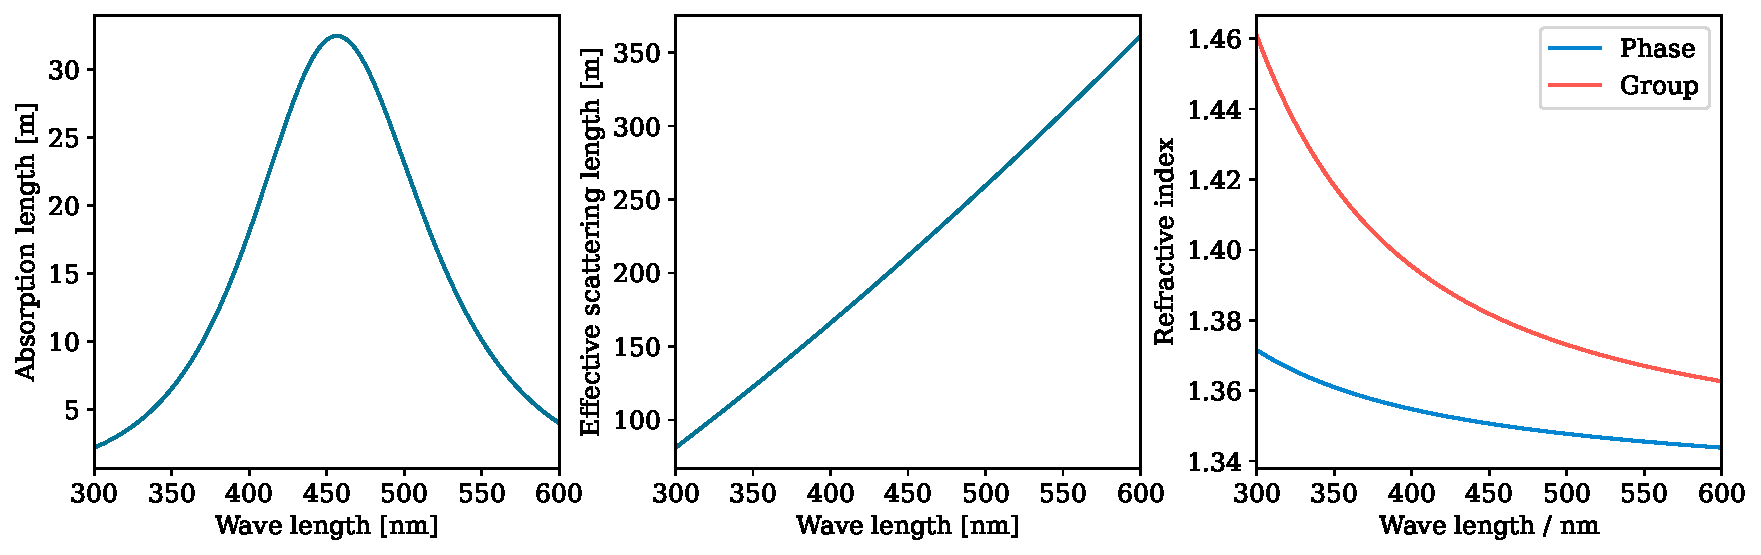
\includegraphics[width=0.95\textwidth]{img/optical_properties_in_simulation.pdf}
    \caption{光子传播模拟中所使用的光学性质参数。}
    \label{fig:optical_properties_in_simulation}
\end{figure}

\subsection{GPU加速的光线传播模拟}
\label{subsec:ray_tracing}

在第二章式\ref{eq:emission_efficiency}中,我们通过简单的估算得到了带电粒子在水中以切伦科夫光的形式辐射的光产额为$\sim 200\, \mathrm{MeV}^{-1}$。那么一个$1\,\mathrm{PeV}$能量的中微子事件如果将能量全部沉积在探测器监控体积内,将会产生$2 \times 10^{11}$个光子。
假设处理追踪一个切伦科夫光子的传播以及与探测器的碰撞需要$\mathcal{O}(10^3)$次的浮点运算次数,考虑现代CPU的运算频率为$\sim 3\,\mathrm{GHz}$,则对一个$1\,\mathrm{PeV}$能量的事件的模拟需要消耗的CPU资源为$\mathcal{O}(10^2) ~ \mathrm{core \cdot hour}$。
如此庞大的计算消耗是服务器集群所难以承受的。

光子在海水的传播以及与探测器的相交过程相比于其他粒子物理模拟在逻辑和运算结构上都是相对简单的,而且在粒子性的框架下不同的光子在传播的过程中并不会相互干扰。
对于这种逻辑简单且可以并行处理的任务而言,可以使用GPU来加速运算。
而且对于光线与物体的相交这种几何运算,在计算机图形学领域已经有大量的研究和现成的软件库可供使用\cite{RT_gems:2021}。
在高能物理领域,也存在不少使用GPU来加速光子传播的应用\cite{Dmitry_PPC:2013, Dmitry_PPC:2022, Opticks:2019, CORSIKA8_GPU:2021}。

在海铃探测器模拟中,我们基于\textsf{OptiX}光线追踪框架实现了GPU加速的光子传播模拟\footnote{\url{https://gitlab.com/hailing/hailing-optix}},其程序的结构图\ref{fig:RT_flow_chart}所示。

\begin{figure}[!htb]
\centering
    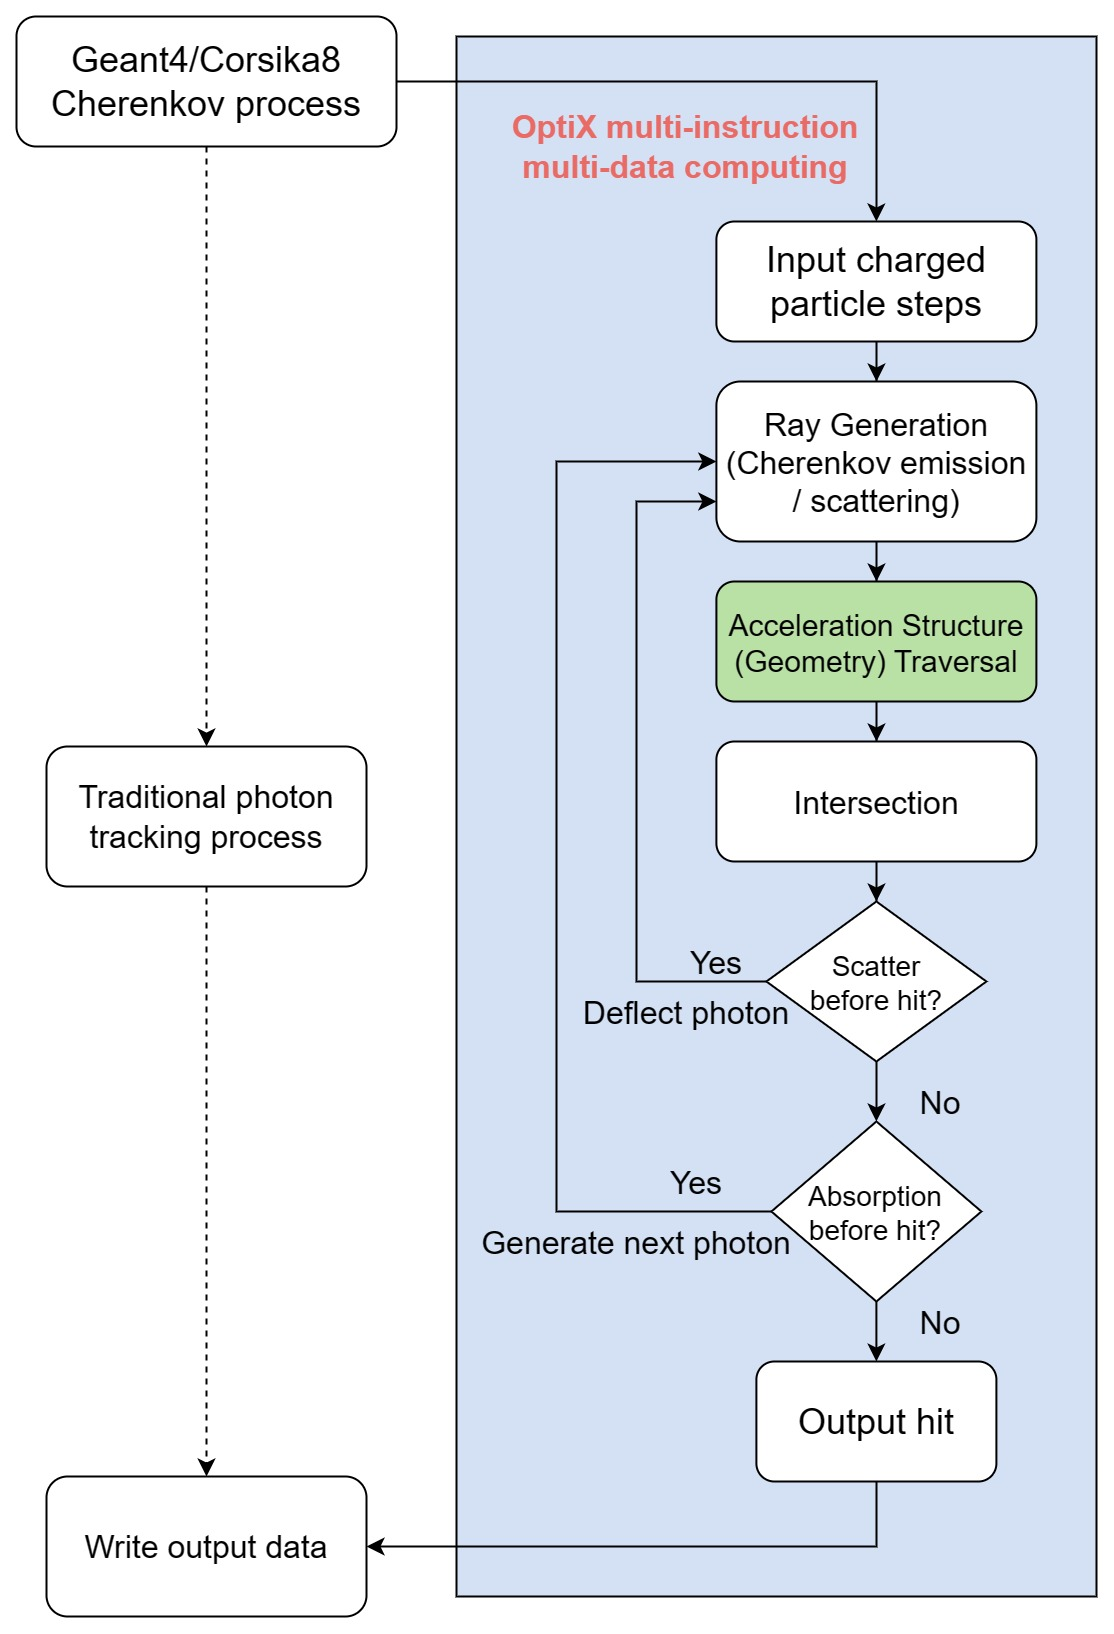
\includegraphics[width=0.75\textwidth]{img/RT_flow_chart.jpg}
    \caption{GPU加速的光子传播模拟的流程示意图。}
    \label{fig:RT_flow_chart}
\end{figure}

在光子传播模块中,我们首先将几何信息传递到GPU程序中。我们将探测器的几何简化为均匀的海水和一个个的DOM球。
光子传播模块从主探测器模拟程序中读取DOM球的几何坐标,并将这约20000个球的坐标位置按照位置的相邻关系构建成方便后续查询的几何加速结构(Acceleration Structure Traversal),从而方便快速地寻找光线与某一个球可能的交点。
海水介质在不同波长上的吸收,散射,折射率等信息被保存在了GPU显存中的材质图上,便于后续的查找和插值。

光子传播模块的输入为\textsf{CherenkovStep}的数组而非切伦科夫光子的数组。在程序中,每一个GPU线程都会各自处理一个\textsf{CherenkovStep}对象。
GPU线程将会根据\textsf{CherenkovStep}的时间,位置,方向,速度信息来不断地通过随机采样的方式产生并传播切伦科夫光子,直到达到该\textsf{CherenkovStep}中所应产生的光子数量。
采用这样的输入模式可以减少GPU显存与系统主存之间的通信开销,因为一个\textsf{CherenkovStep}便对应约1000个切伦科夫光子。
而在GPU计算中,数据传输所占用的时间往往大于真正浮点运算所占用的时间,即GPU计算通常是数据传输受限的(IO bound)\cite{CUDA_for_engineers:2015}。

根据\textsf{CherenkovStep}中的信息产生切伦科夫光子后,程序调用OptiX的光线追踪计算,来判断切伦科夫光子是否与几何体存在交点以及到交点的距离$d_\mathrm{int}$。
紧接着,程序将会根据介质的光学性质以及当前光子的波长来随机采样光子的吸收长度$d_\mathrm{abs}$,散射长度$d_\mathrm{sca}$。
接下来,光子会进行上述三个距离中最短的距离所对应的作用:如果是吸收则开始模拟下一个光子;如果是散射则将光子向前传播$d_\mathrm{sca}$的距离,随后根据散射的相函数改变光子运动方向;如果是相交则表示光子能够击中探测器的表面,我们会将光子在探测器表面的位置,运动方向,波长,以及探测器的ID记录到输出中。
每一个GPU中的线程负责处理一个\textsf{CherenkovStep}中产生的光子,它会不断循环直到将其中应当产生的光子都被处理完全。
此时如果粒子模拟中还有剩余的\textsf{CherenkovStep},则调度中心将会继续为空闲的线程分配新的\textsf{CherenkovStep}。



\section{hDOM探测器模拟}
\label{sec:hdom_sim}

\subsection{hDOM内部的光子传播模拟}
\label{subsec:hDOM_sim}

\begin{figure}[htb]
\centering
    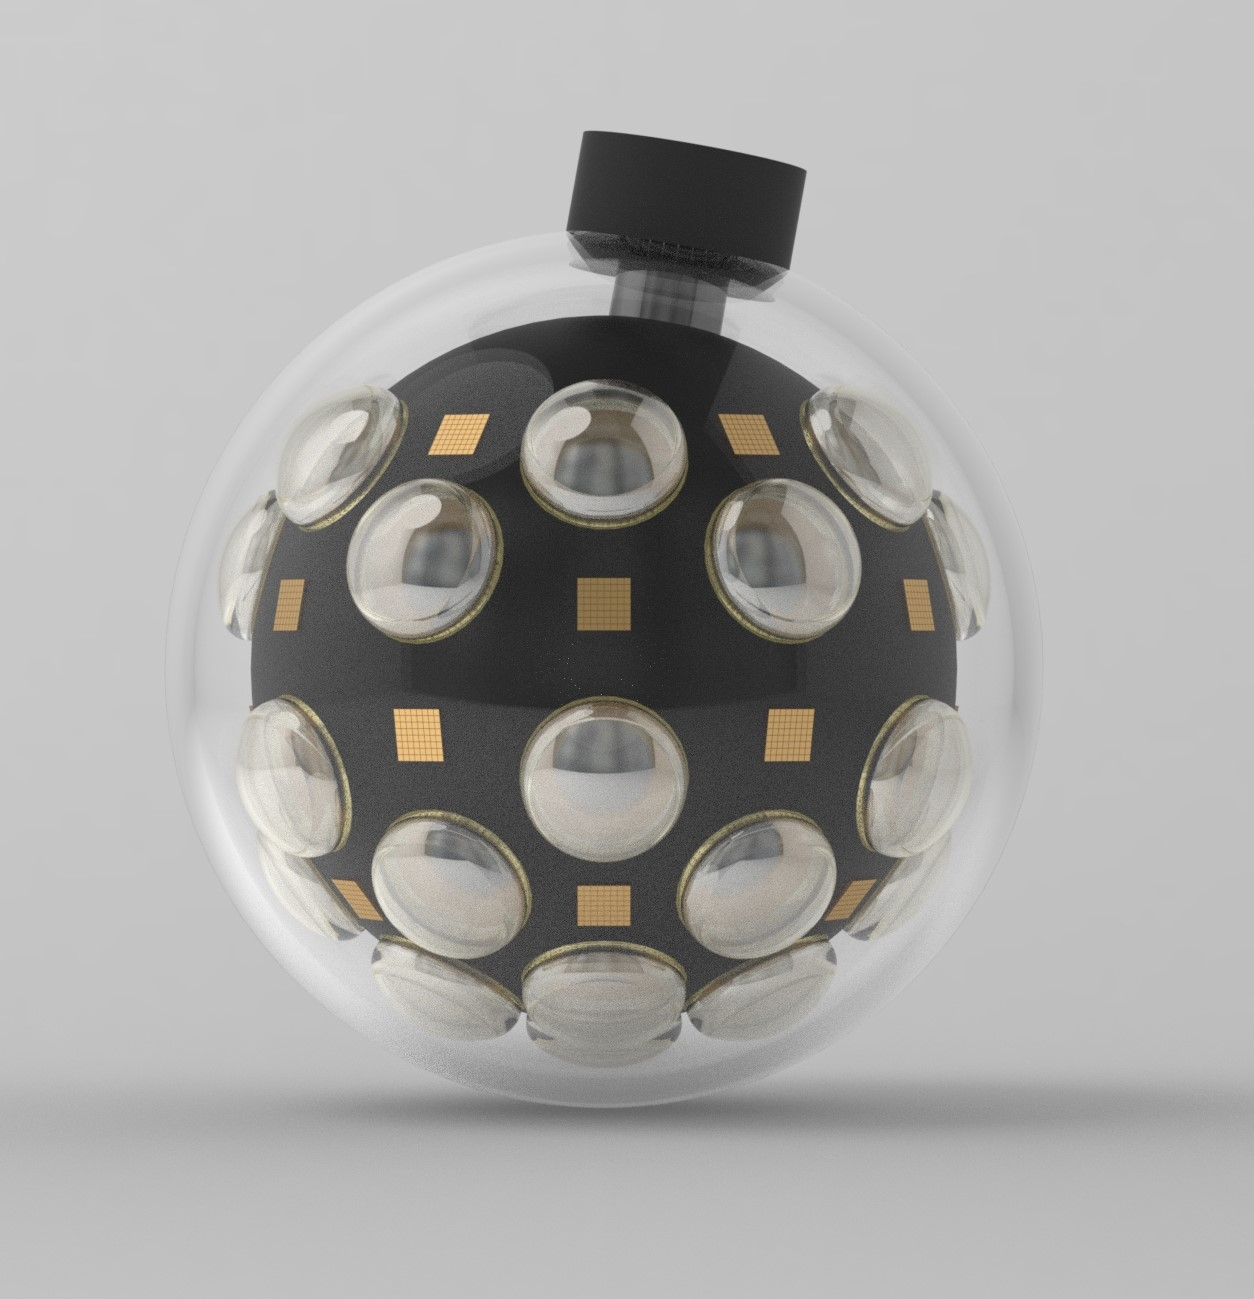
\includegraphics[width=0.7\textwidth]{img/hDOM_rendering.jpg}
    \caption{目前设计的hDOM内部结构的渲染图。}
    \label{fig:hDOM_rendering}
\end{figure}


海铃中微子望远镜的探测单元——hDOM(hybrid Digital Optical Module)的内部结构比较复杂,它包含有PMT和SiPM两种不同的光敏元件。
目前有关PMT和SiPM在探测器内部的几何布局仍然处于积极的研究中,我们需要通过模拟来对比不同排列下的探测器的光子接收面积。
此外,PMT周围的反射环或者光学胶等辅助结构也同样会影响最终PMT的探测效率\cite{IceCube-Gen2_gel_pad:2021}。
因此对于光子在hDOM内部的传播过程的模拟需要一个物理上准确并且可控程度高的程序来处理,在海铃的模拟框架中,我们基于Geant4构建了一个专门的模拟程序\footnote{\url{https://gitlab.com/hailing/hdom}}。
Geant4中存在完整的光子在介质中的吸收和散射,以及光子在穿越不同折射率的介质界面时发生的透射和反射过程。
此外Geant4中还可以通过将几个不同的基本几何体进行交集,并集和补集的操作来构建出复杂而且精细的几何,从而满足未来对探测器内部精细设计的需求。
因此Geant4非常适合对光敏探测元件进行精细的模拟。

我们可以在该程序中构建精细的hDOM内部几何结构,其目前的设计版本所对应的渲染图如\ref{fig:hDOM_rendering}所示。
在当前的设计中,hDOM的最外层是一个17英寸硅硼酸玻璃球壳\footnote{\url{https://www.vitrovex.com/instrument_spheres}},
其外径$21.6\,\mathrm{cm}$,内径$20.2\,\mathrm{cm}$,
密度为$3.0\,\mathrm{g/cm^3}$,折射率为$1.47$。
玻璃球壳内为一个半径为$16.4\,\mathrm{cm}$的不透光的3D打印支架。PMT和SiPM嵌在在3D支架外围。
玻璃球壳和3D支架中间填充着高透明度的光学胶\footnote{\url{https://www.wacker.com/h/en-us/silicone-rubber/silicone-gels/wacker-silgel-612-ab/p/000007546}},其密度为$0.97\,\mathrm{g/cm^3}$,折射率为$1.40$。
光学胶的折射率与外层硅硼酸玻璃以及内部的PMT的玻璃外壳的折射率接近,可以减少光子的界面损失。
在3D打印的支架上安插着31支直径为$3\,\mathrm{inch}$的PMT和24个边长为$\sim 3\,\mathrm{cm}$的SiPM阵列。
这些PMT和SiPM被包裹在凝固之后的光学胶之中,是最终接收探测光子的光敏元件。

在上一步的海水介质的光传播模拟中,光子在hDOM表面的波长和方向信息被记录下来。
这些光子会在hDOM模拟程序中重新发射,光子从hDOM的玻璃球壳外表面处向内传播,如果能够被PMT或者SiPM这样的光敏元件接收,则将其记录下来,作为最终探测器接收到的击中信息。

\subsection{光敏元件响应模拟}

\begin{figure}[htb]
\centering
    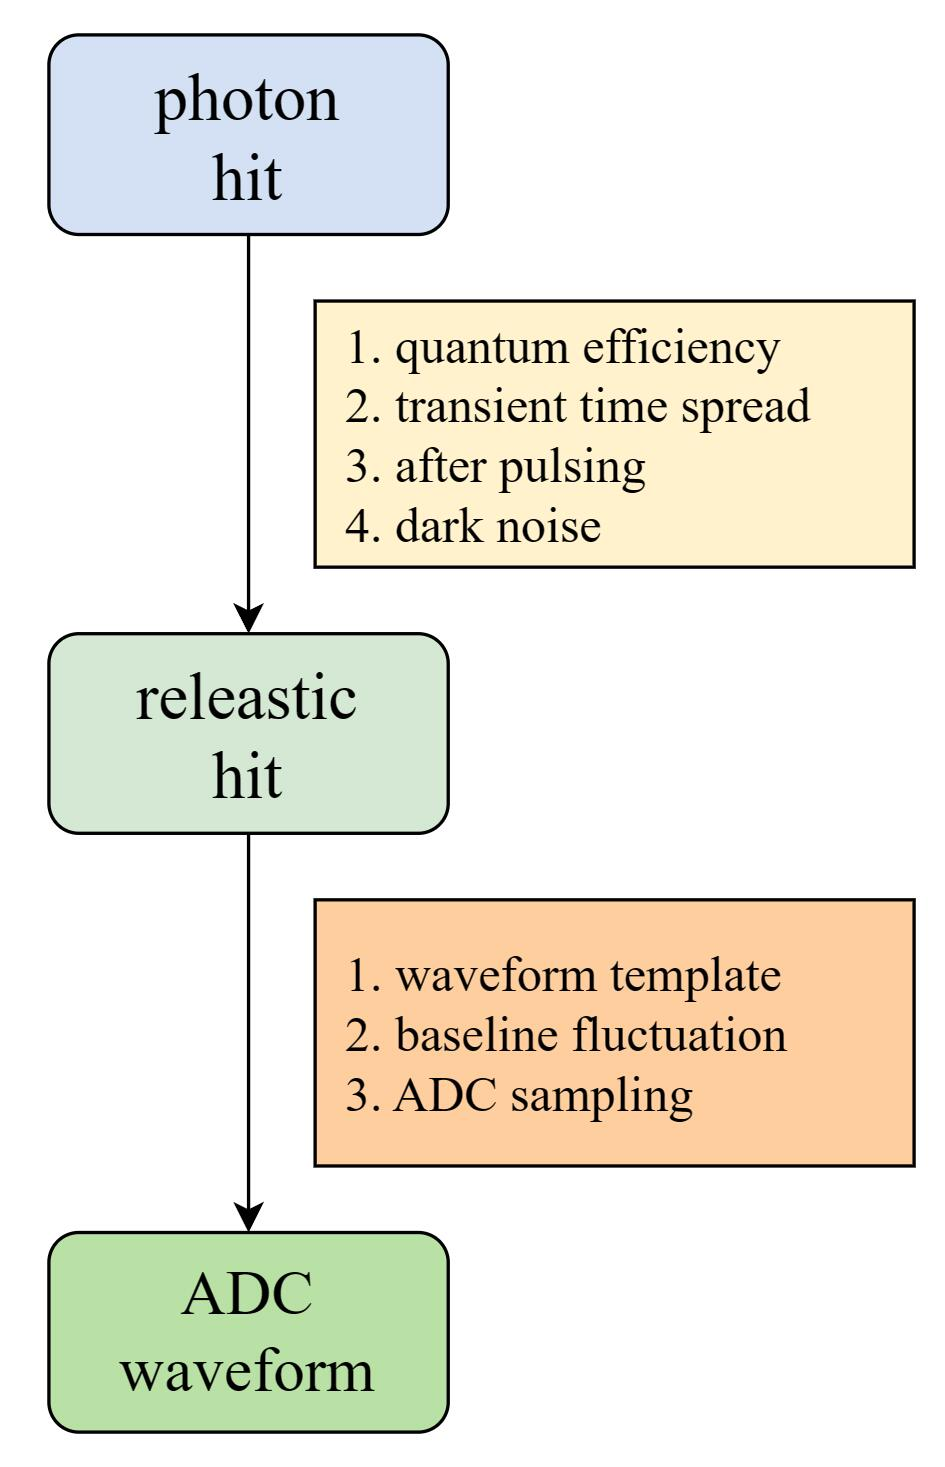
\includegraphics[width=0.5\textwidth]{img/waveform_simulation.jpg}
    \caption{波形模拟程序中的数据流程图。}
    \label{fig:waveform_simulation}
\end{figure}

击中PMT表面的光子,将会经过PMT信号放大成可观测的电信号,随后由模数转换器(Analog Digital Converter,ADC)转换为时间上的电压序列,即波形信号。
我们构建了一个可以模拟PMT对光子的响应的PMT波形模拟程序\footnote{\url{https://gitlab.com/hailing/hailing-wf-simulator}},它可以模拟从光子击中PMT的光阴极到PMT的阳极中输出波形信号以及最终被读数电路放大并数字化的过程,其程序中的数据流如图\ref{fig:waveform_simulation}中所示。

目前该程序的功能框架已经完备,但具体PMT的详细物理性能还有待测试,电子学读数电路尚未制作完成,其性能要求也仍在评估中。

从理论上来说,SiPM对光子的响应波形与PMT类似,具体而言SiPM会拥有更好的时间分辨能力,量子效率以及单光子分辨率,但同时也会有更严重的暗噪声和串扰现象。
由于我们实验团队对SiPM自身的硬件性能测试还处于早期阶段,因此对模拟SiPM响应的模拟程序暂未开发。
